\section{Technical Approach}
\label{sec:TechnicalApproach}

\begin{figure}
\centering
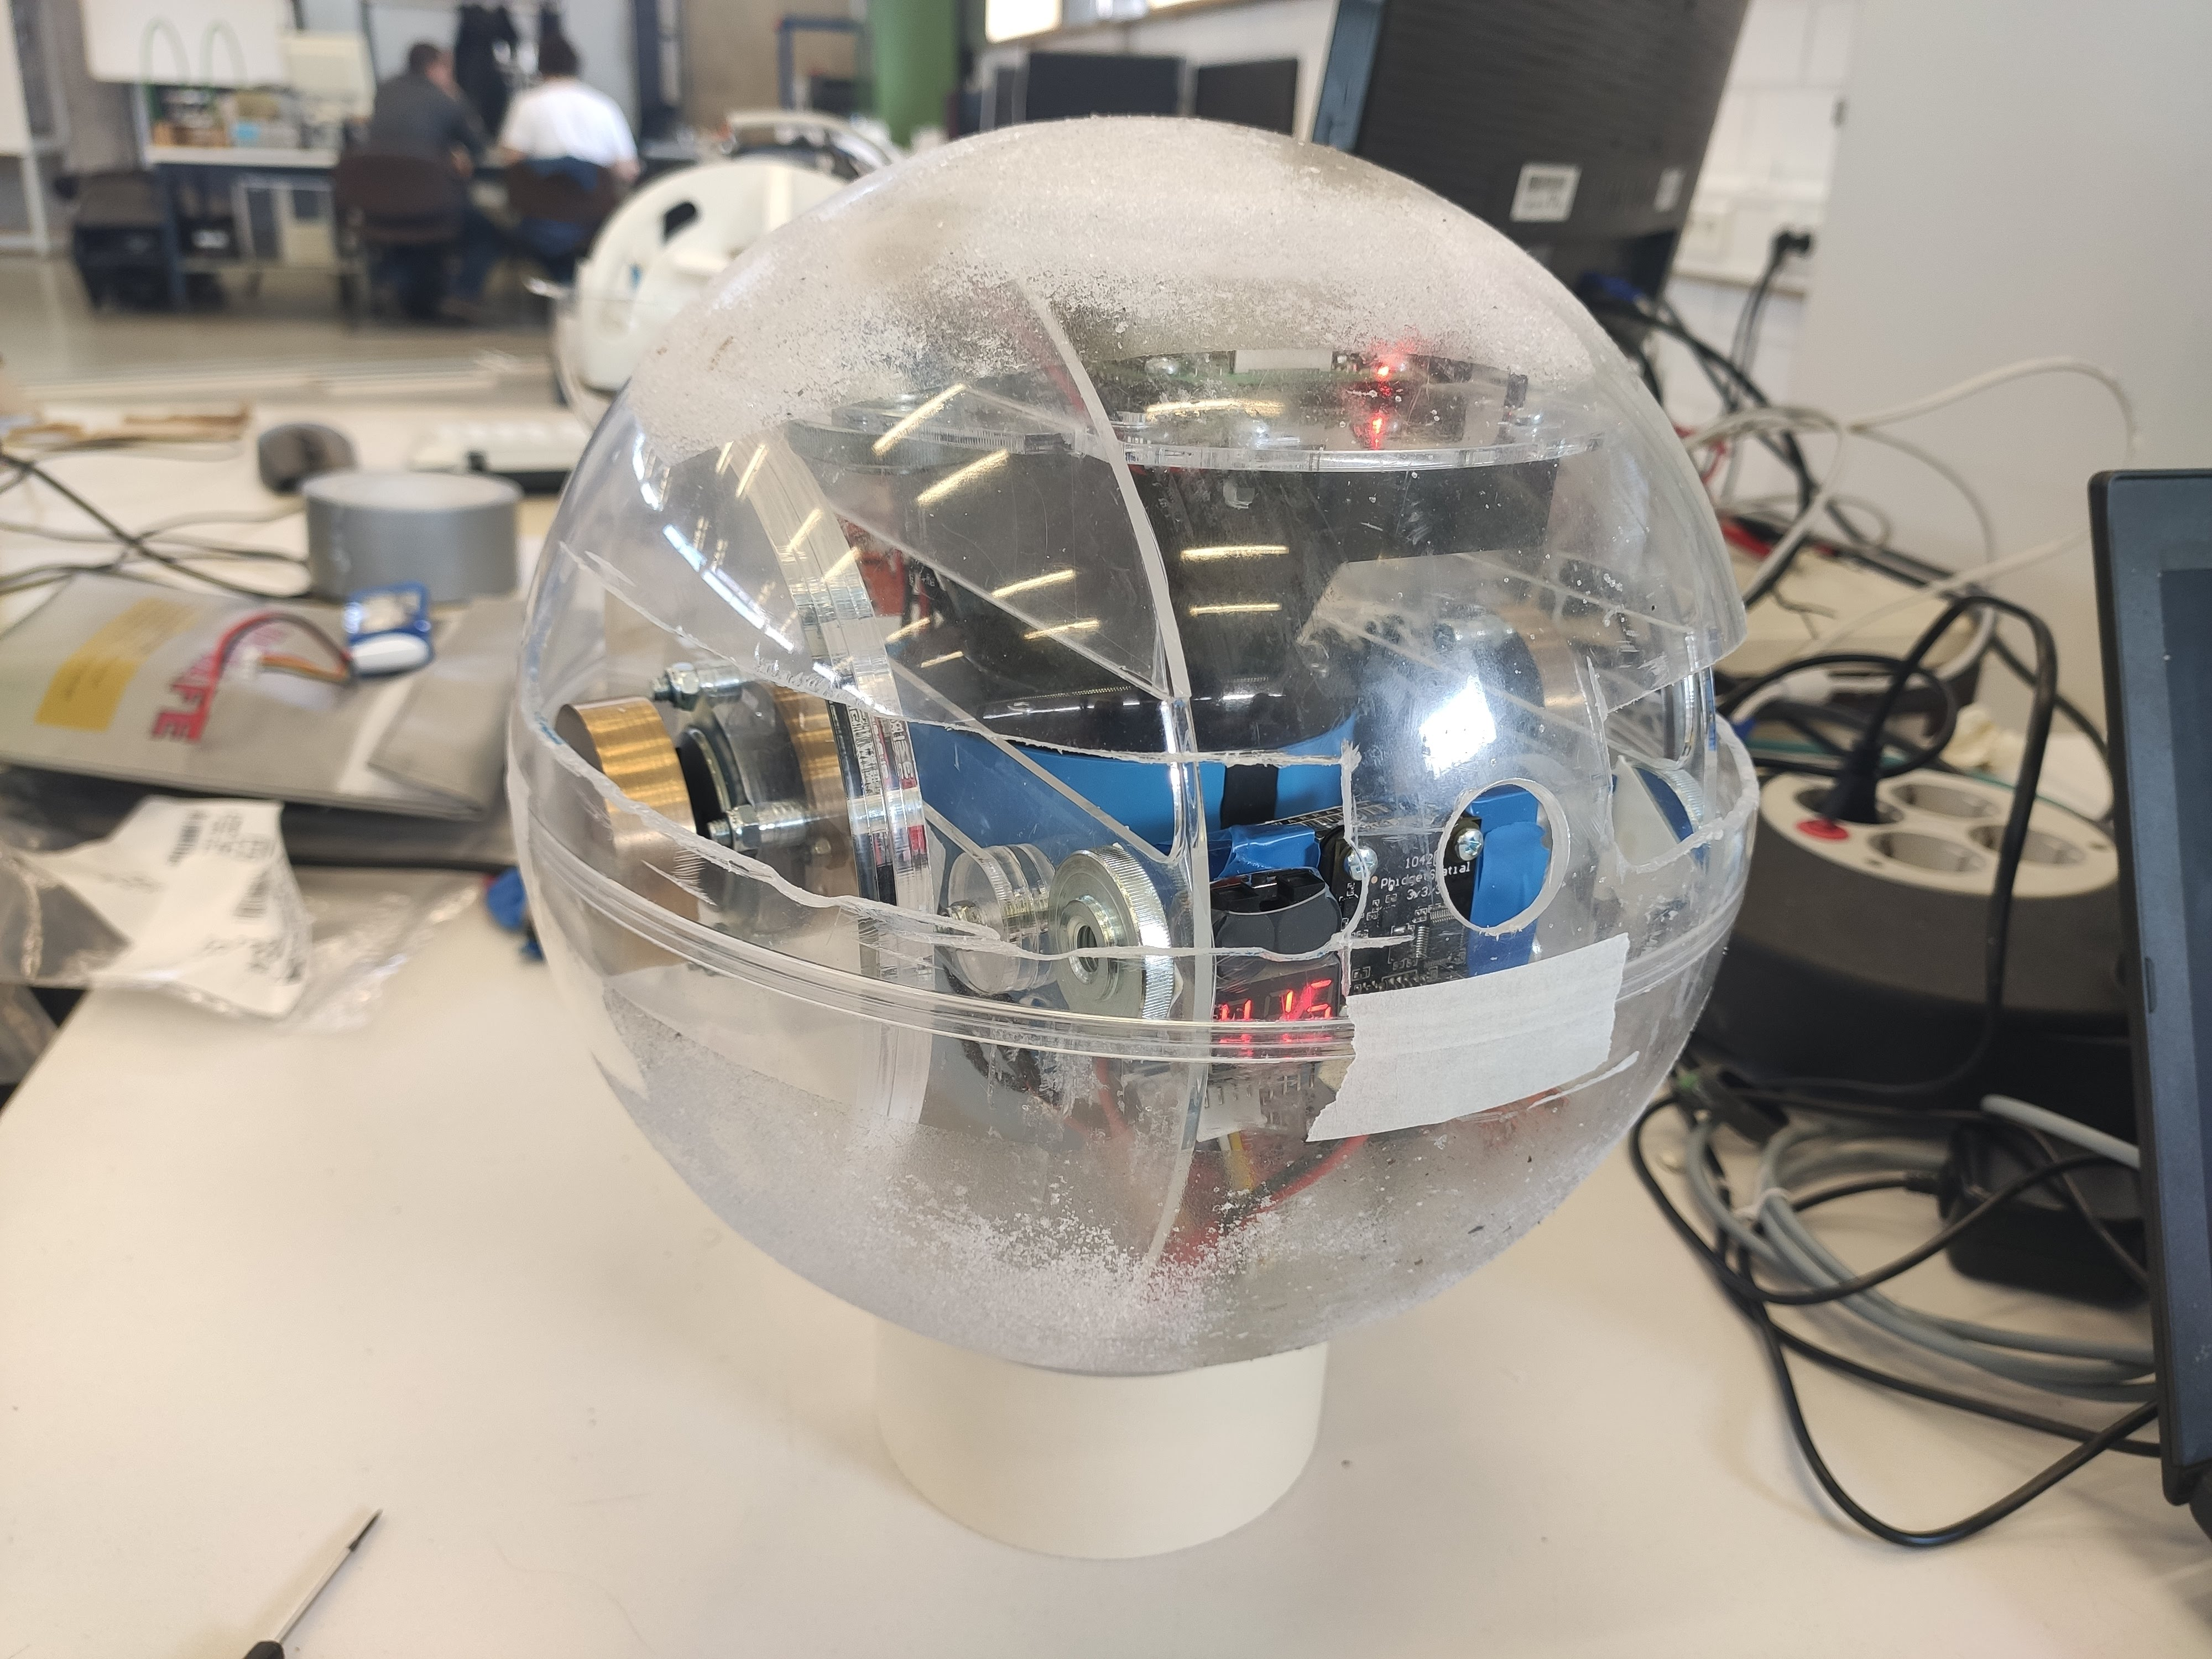
\includegraphics[height=55mm]{../Media/sphereFullshellLeft.jpg}
\hfill
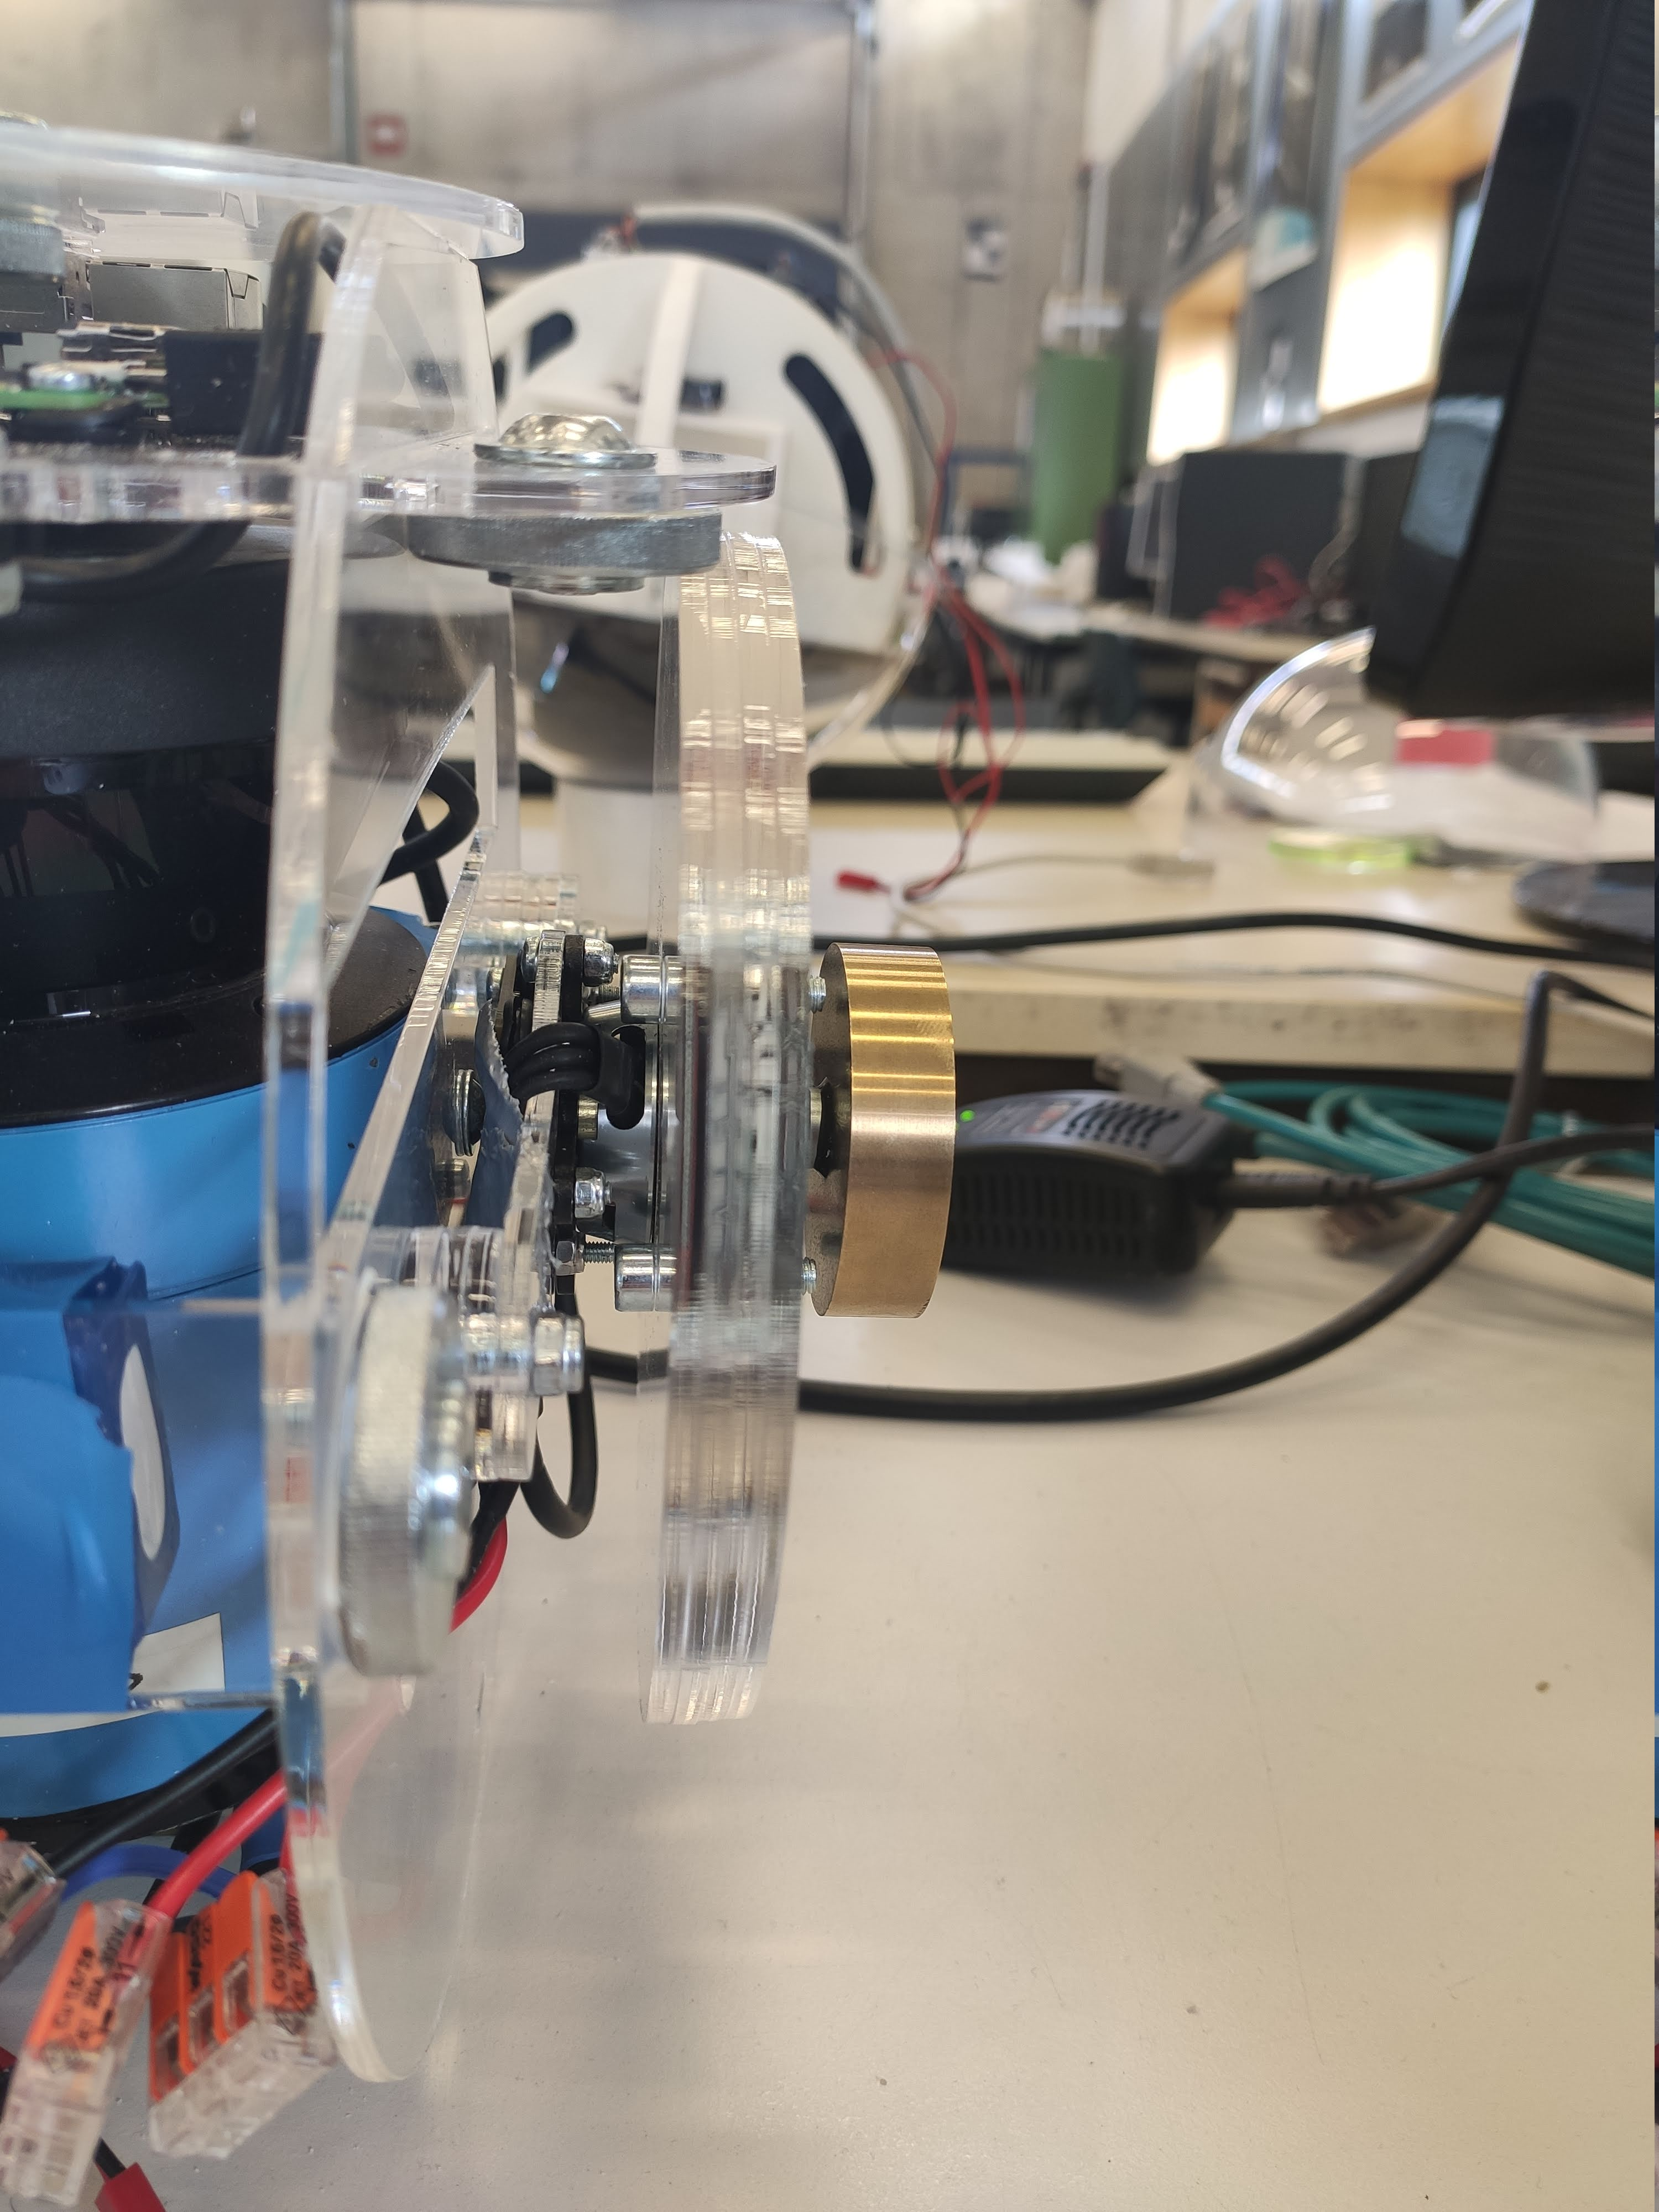
\includegraphics[height=55mm]{../Media/sphereRightMotor.jpg}   
\caption{Hardware setup of the L.U.N.A sphere prototype, including notches in the shell and friction granule (left). IMU (beneath supporting structure) and brushless motor  including flywheel mass (above supporting structure) of the L.U.N.A sphere (right).}
\label{sec:TechnicalApproach:fig:setup}
\end{figure}

\todo{Wie dreht sich die Kugel überhaupt ? COAM + Cubli paper lesen / gyro effekt + video schneiden (ohne ton) }

Figure \ref{sec:TechnicalApproach:fig:setup} shows the final hardware setup of the robot.
\todo{was ist da drinnen (raspberry pi, ..), wo ist es da drinnen, warum ist es da drinnen.}
In order to reduce complexity with respect to the 3D-transformation calculations, the laserscanner was placed at the center of a spherical acrylic glass shell as precisely as possible.
This limits the laser scanners movement to rotational movement and removes translational movement completely. With this initial setup given, the only room left for the acrylic glass structural components, batteries, boardcomputer, IMUs, motors, weights and wiring are the spaces between the scanner and the shell. On each side one Turnigy Park480 brushless outrunner motor \cite{turnigymotor} of the COAM drive with two flywheels is attached.
Strong epoxy glue attaches the weights to the motor shafts and shells.
As the flywheels start spinning with respect to the structural components of the sphere, the sphere itself starts spinning with respect to the ground. 

Figure \ref{sec:TechnicalApproach:fig:setup} also shows that the top and the bottom of the shell are covered in table salt, which made a good granule to increase friction to the ground in the early testing phase. Furthermore, there are notches in the front side of the shell to increase permeability for the laser.
Unfortunately, the laser scanner measurements are still affected by blockades due to components of the sphere.
Specifically, the outside shell is an inhibiting factor as an object with the distance of the radius is measured at all times, \todo{which is why measurement slits}
                                                                                                                                                                                                                  
\begin{figure}                                                                                                                                                                                                    
\centering                                                                                                                                                                                                        
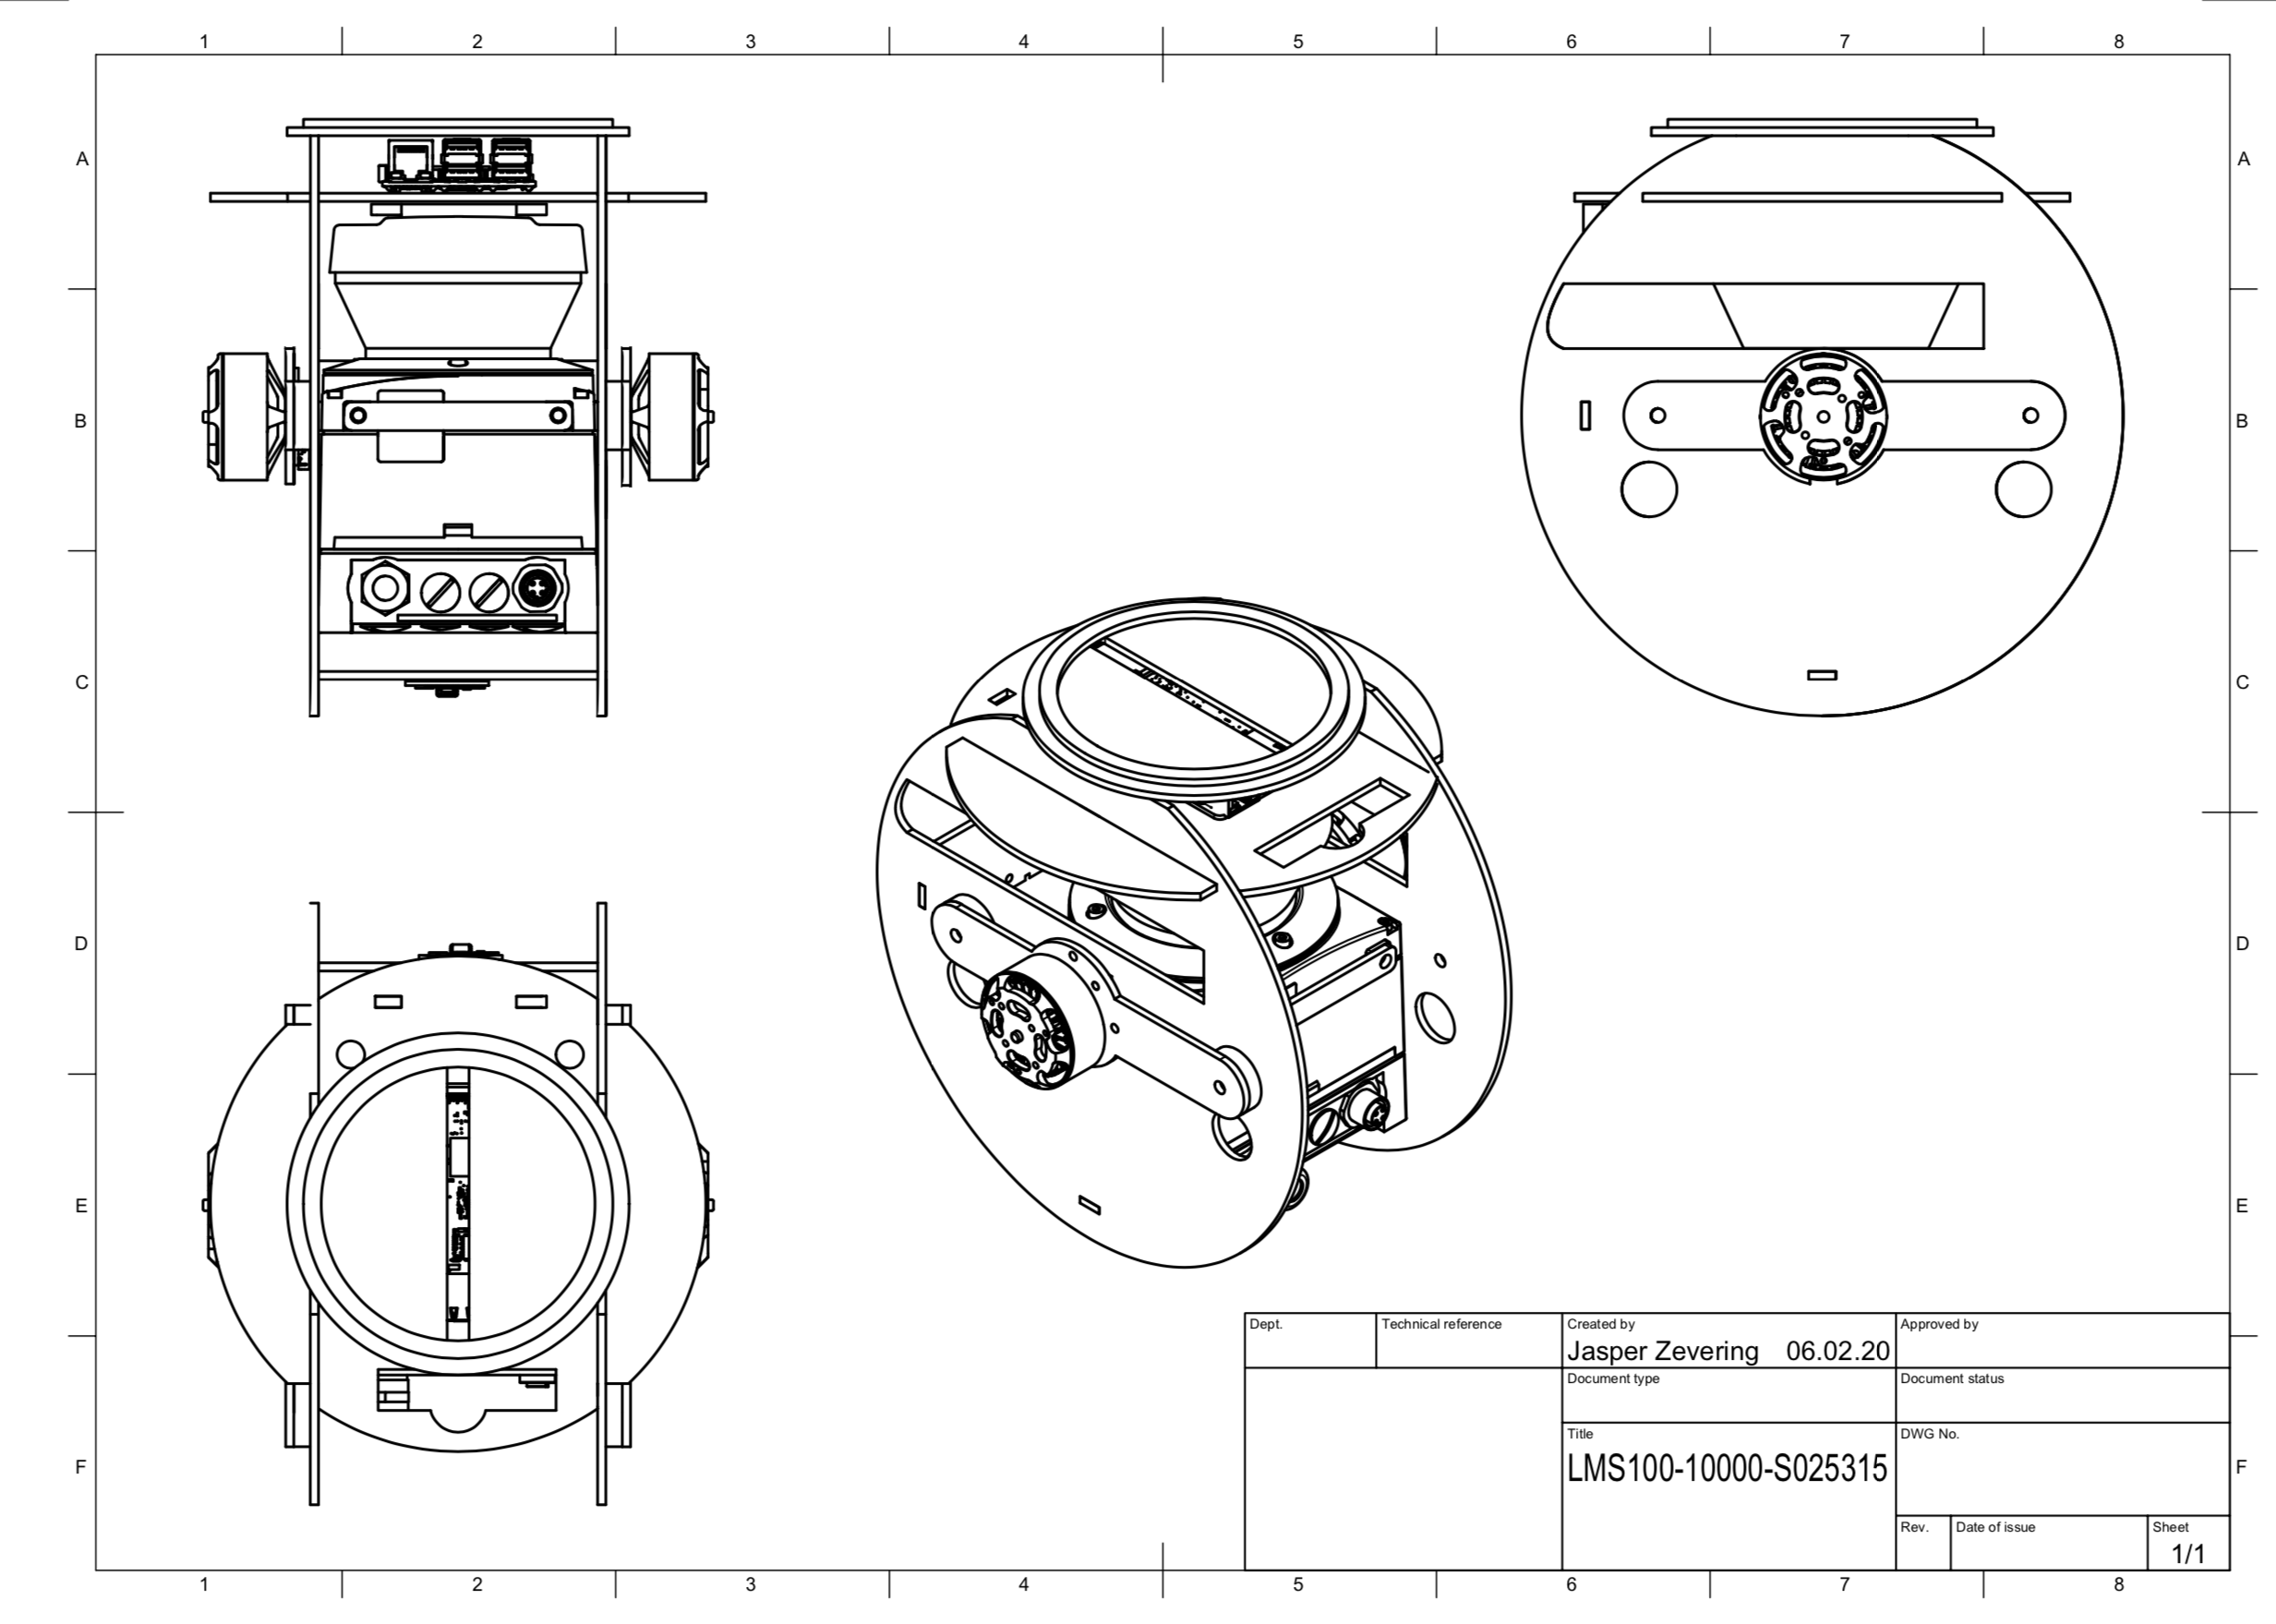
\includegraphics[width=\textwidth]{../Media/BlueprintPNG.png}                                                                                                                                                      
\caption{Blueprint of the mechanical structure of the spherical robot.}                                                                                                                                   
\label{sec:TechnicalApproach:fig:blueprint}                                                                                                                                                                       
\end{figure}                                                                                                                                                                                                      
                                                                                                                                                                                                                  
Figure \ref{sec:TechnicalApproach:fig:blueprint} shows a CAD blueprint of the overall interior layout of the mechanical structure of the L.U.N.A sphere, ignoring the outside sphere, flywheels and wiring.
The payload is mounted to supporting structural components which are made of acrylic glass.
The Raspberry Pi 3B boardcomputer is placed on top of the laser.
Above that, another supporting structure holds additional counterweights to correct for inhomogeneous weight distribution.                                                                                                     
The battery finds its place in front of the laser scanner on another supporting structure.
The two brushless motors were each placed on one side of the supporting structure with spacers that leave room for the side IMU underneath one of the motors.
Two other IMUs are placed in front of and beneath the laser to ensure coverage of all axes.                                                                                 

\begin{figure}                                                                                                                                                                                                    
\centering
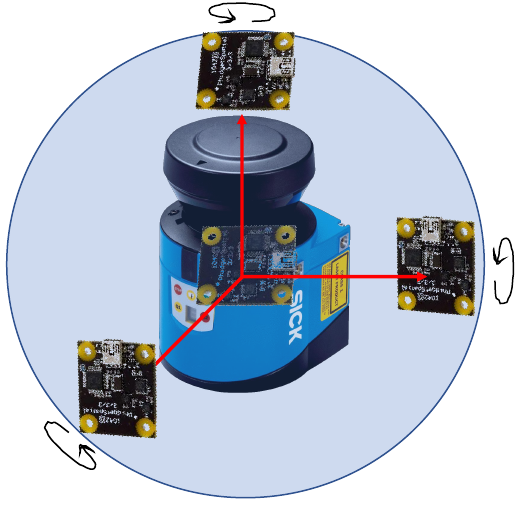
\includegraphics[width=0.4\textwidth]{../Media/virtualIMU.png}                                                                                                                                                      
\caption{Sketch that helps illustrate the combination of 3 IMUs into 1 virtual IMU that simulates being at the center of the sphere.}                                                                                                                           
\label{sec:SensorIntegration:fig:virtual}                                                                                                                                                                       
\end{figure}                                                                                                                                                                                                      

\subsection{Sensor Integration}
\label{sec:TechnicalApproach:sensorintegration}

The sensor integration is fully implemented with the Robot Operating System (ROS) using the Ubuntu distribution \href{http://wiki.ros.org/ROSberryPi}{ROSberryPi} which contains a pre-installed ROS version.
Overall, three seperate PhidgetsSpacial 10441B IMUs \cite{imuphidgets} keep track of the pose of the sphere. Each IMU is placed in such a way that the IMUs Z-axis corresponds to one possible rotation axis of the sphere.
Therefore, each IMU is perpendicular to the other two.
Combining the axes measurements leads to a "virtual" IMU, which emulates being an IMU positioned at the center of the sphere. 
Hence, isolating the measurements of the resulting virtual IMU to only the rotation in the given axis.
Figure \ref{sec:SensorIntegration:fig:virtual} illustrates this principal.
Previous prototypes have shown that transforming the data of only one non-centered IMU leads to lower quality measurements.
However, combining the measurements of three IMUs, where each measures only the static rotation around one of their rotational axes (which also represents a rotation axis of the sphere), leads to less noise, as seen in figures  \ref{sec:technicalApproach:fig:imu1_ang_vel}-\ref{sec:technicalApproach:fig:merged_ang_vel}.

\begin{figure}
\centering
\begin{subfigure}{0.45\textwidth}
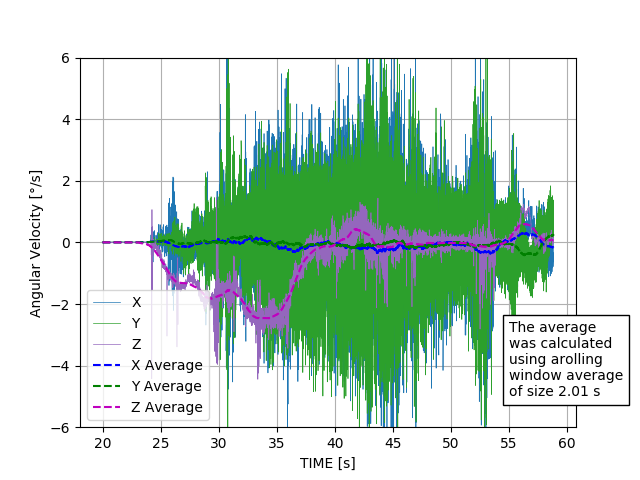
\includegraphics[width=\textwidth]{./plotsAndScripts/angVel-2020-01-29-16-14-54/imu1_ang_vel}
\caption{IMU 1: Z-Axis corresponds to Sphere X-Axis}
\label{sec:technicalApproach:fig:imu1_ang_vel}
\end{subfigure}\hfill
\begin{subfigure}{0.45\textwidth}
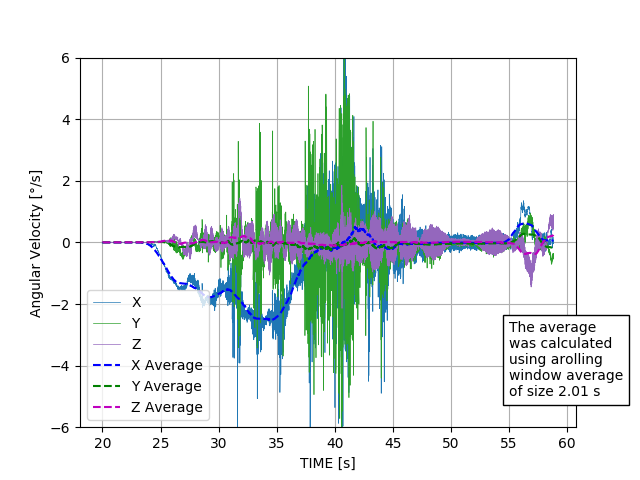
\includegraphics[width=\textwidth]{./plotsAndScripts/angVel-2020-01-29-16-14-54/imu2_ang_vel}
\caption{IMU 2: Z-Axis corresponds to Sphere Z-Axis}
\label{sec:technicalApproach:fig:imu2_ang_vel}
\end{subfigure}\hfill\\

\begin{subfigure}{0.45\textwidth}
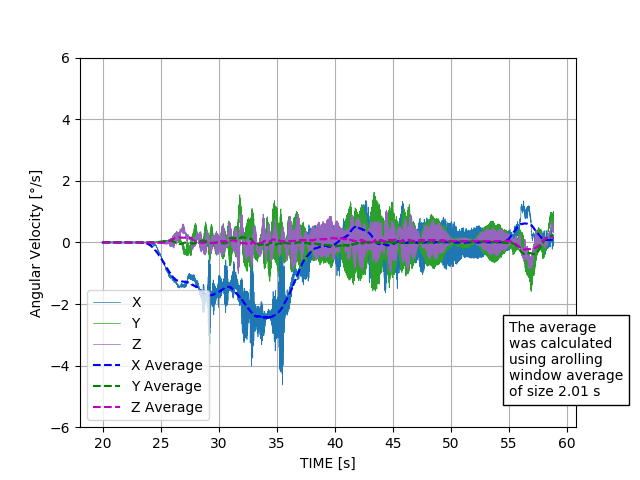
\includegraphics[width=\textwidth]{./plotsAndScripts/angVel-2020-01-29-16-14-54/imu3_ang_vel}
\caption{IMU 3: Z-Axis corresponds to Sphere Y-Axis}
\label{sec:technicalApproach:fig:imu3_ang_vel}
\end{subfigure}\hfill
\begin{subfigure}{0.45\textwidth}
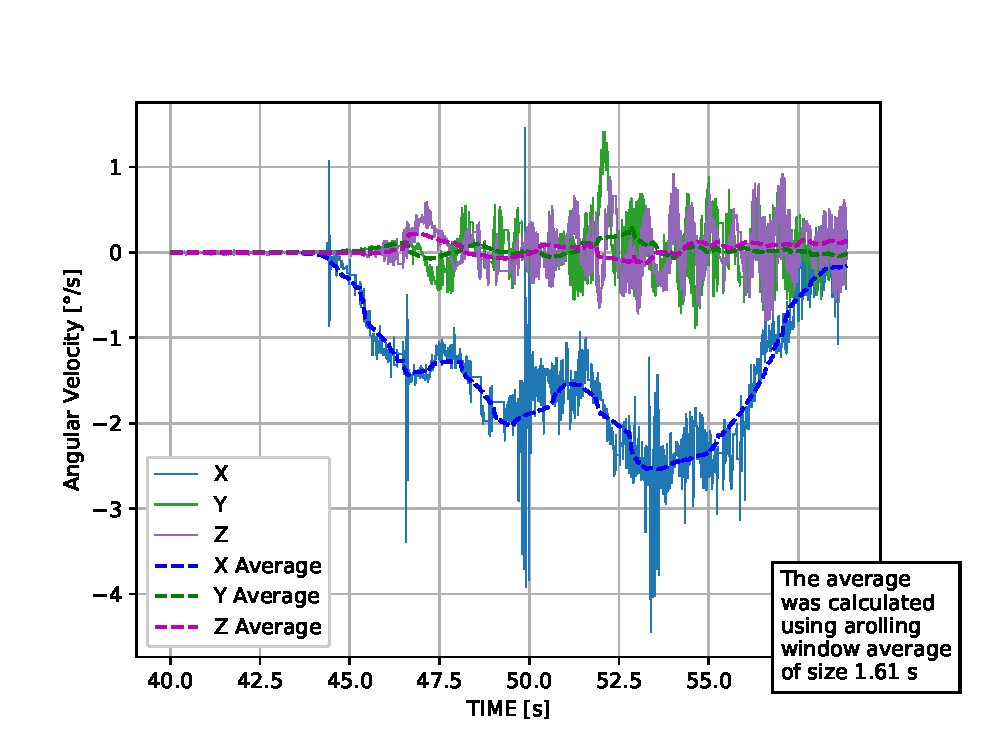
\includegraphics[width=\textwidth]{./plotsAndScripts/angVel-2020-01-29-16-14-54/merged_ang_vel}
\caption{Merged virtual IMU. Maps the Z-Axis of all other IMUs to the rotational axes.}
\label{sec:technicalApproach:fig:merged_ang_vel}
\end{subfigure}\hfill
\caption{Angular velocity measurements of singular IMUs and the combined IMU.}
\label{sec:technicalApproach:fig:angvel}
\end{figure}

The IMUs also ship with accelerometers that are used to determine the full pose of the sphere.
Each IMU calculates their pose separately, using a quaternion extended Kalman filter (QEKF).
However, combining those poses into one does not have any positive effect, but only makes the software more resource demanding and slow.
Thus only the pose of the bottom IMU's accelerometer is used to keep track of the pose.

The motors are controlled using the piGPIO library. The GPIO signals are forwarded by the pins to two ESCs that drive the motors. 

Unfortunately, the brass weights are not drilled in the very center, causing an unbalance when rotating.
The resulting vibrations inhibit the movement of the sphere.
Thus a controller was implemented that measures the extend of the vibrations using standard deviations of the non-rotating axes of the IMU and adjusts the throttle of the motors accordingly.
This was done with a two-point controller with hysteresis.
Considering the translational velocity of the sphere in a controller is not possible.
The speed of the sphere is calculated by the rotational speed, which is why slippage of the sphere causes such a controller not to produce the desired motion. 

\subsection{Point Cloud Processing}                                                                                                                                                                                  
\label{sec:TechnicalApproach:pointcloudprocessing}
For the processing of the point cloud the 3D Toolkit (3DTK) was used.
This provides multiple methods and algorithms for processing 3D point clouds, especially the 6D continuous time Simultaneous Localization And Mapping (SLAM) algorithm (see \cite{3DARCH2017_1, LS2019}) as post-processing.
Therefore only the time-stamped raw data of the IMUs and laser-scanner is transferred and the estimation of the pose and the SLAM algorithm itself is performed externally.
For this prototype the transfer is realized using the host-function of ROS, giving the external PC the possibility to subscribe to the topics and process them.
3DTK itself takes pairs of files, one representing the pose, one the laser scanner data, and each file named by the time-stamp with an identifier if it is scan-data or pose.
Also, the use of USB-connected IMUs and ROS as transfer-mechanism of data leaves potential for enhancement and therefore reducing the load of the internal controller.